\section{Reaching Definitions Analysis}

Analisis \compiler{Reaching Definitions} adalah analisis \textbf{Forward} dengan meet operator \textbf{Union} ($\cup$). Analisis ini menentukan definisi (penugasan nilai) mana yang mungkin masih aktif saat mencapai titik program tertentu.

\subsection{Persamaan Aliran Data}
Untuk setiap blok $B$, hubungannya didefinisikan sebagai:
\begin{enumerate}
    \item \textbf{Meet Operation}: $IN[B] = \bigcup_{P \in Pred(B)} OUT[P]$ (Definisi yang mencapai awal blok adalah gabungan dari semua yang keluar dari pendahulunya).
    \item \textbf{Transfer Function}: $OUT[B] = GEN[B] \cup (IN[B] - KILL[B])$.
\end{enumerate}

Di mana:
\begin{itemize}
    \item $GEN[B]$: Himpunan definisi yang dibuat di dalam blok $B$ dan mencapai akhir $B$.
    \item $KILL[B]$: Himpunan definisi di luar $B$ yang variabelnya di-assign ulang di dalam $B$.
\end{itemize}

\subsection{Konsep Fixed-Point}
Kompilator menjalankan algoritma ini secara berulang di seluruh CFG. Karena himpunan data hanya bisa bertambah (monotonik) dan jumlah definisi terbatas, algoritma dijamin akan berhenti pada suatu titik di mana nilai $IN$ dan $OUT$ tidak lagi berubah. Titik stabil ini disebut \textbf{Fixed-Point}.

\begin{figure}[!htbp]
    \centering
    \adjustbox{max width=0.8\textwidth,center}{%
    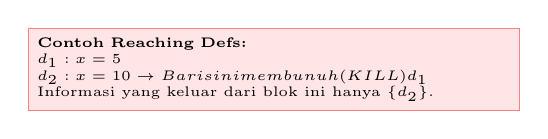
\begin{tikzpicture}[
        rect/.style={rectangle, draw=red!50, fill=red!10, text width=6cm, font=\tiny}
    ]
    \node[rect] (eq) {
        \textbf{Contoh Reaching Defs:}\\
        $d_1: x = 5$\\
        $d_2: x = 10 \to \text{Baris ini membunuh (KILL) } d_1$\\
        Informasi yang keluar dari blok ini hanya $\{d_2\}$.
    };
    \end{tikzpicture}%
    }
    \caption{Ilustrasi Operasi GEN dan KILL}
\end{figure}
